% This report uses the
% LLNCS macro package for Springer Computer Science proceedings;
% Version 2.20 of 2017/10/04
%
\documentclass[runningheads, 12pt]{llncs}
%
\usepackage{graphicx}
% Used for displaying a sample figure. If possible, figure files should
% be included in EPS format.
%
% If you use the hyperref package, please uncomment the following line
% to display URLs in blue roman font according to Springer's eBook style:
% \renewcommand\UrlFont{\color{blue}\rmfamily}

\begin{document}
%
\title{Coursework 2 - Data Mining}
%
%\titlerunning{Abbreviated paper title}
% If the paper title is too long for the running head, you can set
% an abbreviated paper title here
%
\author{David Frame - 40200819}
%
\authorrunning{D. Frame}
% First names are abbreviated in the running head.
% If there are more than two authors, 'et al.' is used.
%
\institute{Edinburgh Napier University\\
\email{40200819@live.napier.ac.uk}}
%
\maketitle              % typeset the header of the contribution
%
\section{Introduction}
In this report, we will discuss the results of data preparation and mining for data analytics. This involves cleaning the data, converting it into a use-able format and analyzing it using various algorithms.

%The abstract should briefly summarize the %contents of the paper in
%150--250 words.

%\keywords{First keyword  \and Second keyword %\and Another keyword.}

% REFERENCE STUFF \ref{distJumpLocBMen}
%
% DESCRIPTION OF RELATIONSHIPS
\section{Data Preparation}

To prepare the data for analysis, the author cleaned the data and exported it into mixed and nominal only data sets in arff format. The author initially planned to also create a numerical only version, but this wasn't needed for the algorithms used. The cleaning and preparation processes are explained in further detail in this section.

\subsection{Data Cleaning}

The author used OpenRefine to clean the data. To start, the column names were added as they were missing from the data set. This made it easier to find errors and mistakes, For example, naming the age column made it clear that some values were wrong, such as negative or decimal numbers.

The text facet option was used to find spelling errors and duplicates that they cause, as well as data type issues such as numbers being stored in text format.

Some decisions needed to be made, such as what to do with 'yes' in the job column as this wasn't an available option. It was clear that it would be categorized as either high qualif/self emp/mgmt, unskilled resident or skilled. The skilled category was chosen as it was a middle ground between highly skilled and unskilled, it was also the most common option, increasing the likelihood that it accurately represents the data.

Similarly, the personal status attribute had a value 'female div/dep/mar', which was assumed to be a typo as the description was 'Female Divorced/Separated/Married'. Therefore, the value was changed to 'female div/sep/mar'.

The credit amount attribute had some outliers, with values breaching 120 million in some cases. To address this, a more appropriate number for each outlier was found by comparing rows with a matching purpose; for example, if all rows with a purpose of 'new car' had credit amount values in the 10000s, some zeroes would be removed from the outlier to bring it closer to the expected value range.

\subsection{Data Conversion}

After the data had been cleaned, the author created 2 versions of the data: The original data and a nominal only version. A numerical only version was also planned, but ultimately wasn't required for the algorithms used. 

To create the nominal version, all numerical values were changed to text strings that grouped them in logical ways, for example the age column was categorized into child, young adult, adult and senior. The case number column was removed as it wasn't being used for anything and it had a numerical datatype.

Each version of the data was exported from OpenRefine to an Excel file, opened in Excel and converted into a CSV file. After this, the CSV files were edited in Notepad to change them into arff format. This involved labelling the column names with '@attribute' and following them with a suitable data type. The rest of the data was labelled with '@data' before saving the file in arff format.

After this process, the datasets were ready to analyze in Weka.

\section{Data Analytics}

Weka was used to analyze the data for this project. This involved running various algorithms to find rules about the data, as described below.

\subsection{Classification}

To find rules with classification techniques, the author employed the use of the j48 algorithm with the cross validation option  selected (with 10 folds). The author tried using both the nominal and standard versions of the data set yet there was no perceived change to the results, so either can be used to recreate the following rules. 

This produced a large tree with many leaves, with the initial split based on the checking status attribute. To consolidate the tree into a more manageable size, the minimum number of objects was increased from 2 to 10. 

There were a few rules to find in this tree, the most prominent one being for those with a checking status of 'no checking', which has a score of 394/46. With 394 matching the rule and only 46 getting a bad rating, this makes the rule accurate for 89.5\% of the data.

Those with a checking status less than 0 and a credit history of 'critical/other existing credit' have a very high chance of a good rating (67/18, 78.8\%). Similarly, those with a checking status of '\textgreater=200' also have a very high chance of a good score (63/14, 81\%).

Those with a checking status of '\textless0', credit history of 'existing paid' and purpose of 'furniture/equipment' are likely to receive a good rating, with a score of 45/17 or 72.6\%. A similar result occurs with the same parameters, but with 'new car' as the purpose instead - giving a score of 42/15 or 73.7\%.

Conversely, those with a checking status of '\textless0' and a credit history of no credits/all paid are likely to receive a bad rating, with a score of 13/3 or 81.3\%. This is admittedly a small pool of data, and the result seems harsh for those with a credit history of 'no credits/all paid' as they have no negative history with the bank. For these reasons, this rule may be an anomaly.

After making the above observations, the author changed the minimum number of objects to 60, to see which checking status values were the most influential on the credit rating. The resulting tree shows that those with a checking status of '\textgreater=200' have a very high chance of a good rating, with a score of 63/14 or 83.1\%. Checking status values of '0\textless=X\textless200' are less certain by comparison, only having a score of 269/105, or 72\%. Overall, a checking status of '\textless0' gives the highest likelihood of a bad rating whilst '\textgreater=200' gives the highest  chance of a good rating.

\subsection{Association}
To find rules by association, the Apriori algorithm was used with the nominal version of the data set. Starting with standard settings, there were no rules generated pertaining to the value of the class attribute. To remedy this, the minimum confidence was gradually lowered until some relevant rules were generated (at a confidence minimum of 0.7). The rule with the highest confidence states that those with a credit amount less than 5000 are likely to get a good rating, with a confidence level of 74\%. Interestingly, the next rule states that those with a credit amount value less than 5000 who are adults specifically are also likely to receive a good score, with exactly the same confidence rating (74\%).

Many other rules follow this pattern, with single males having a 73\% change of a good rating, a confidence rating which remains the same if they are specifically adults. This implies that age has no effect on rules that follow this pattern.

Some other rules to be found using the Apriori algorithm include the fact that those with skilled jobs have a 70\% chance of a good rating, adults have a 70\% chance of a good rating, those with a credit history of existing paid have a 68\% chance of a good rating and those with a saving status of '\textless100' have a 64\% chance of a good rating. 

Unfortunately, the rules with very high confidence values don't imply a value for the class attribute. For example, those with a skilled job and a class value of good are likely to be adults, with a 94\% confidence. Predicting the likelihood that a person is an adult obviously isn't too useful in this case. The author attempted to infer that those who are adults with a skilled job also have a 94\% confidence for a good rating, but this is not the case as we already mentioned that skilled adult workers have a 70\% chance of a good rating - proving that these rules don't work in both directions.

\subsection{Clustering}
After adjusting some settings, the author found that using the SimpleKMeans algorithm with the nominal data set, a seed of 11 and the 'use training set' option created 2 clusters, one with a good class rating and one with a bad rating. This allows general rules to be found about which variables affect the result the most.

For example, the good cluster has an average employment level of '\textgreater=7, which is quite a lot higher than '1\textless=X\textless4' for the bad cluster. This indicates that more experience increases the chances of a good rating, which makes logical sense. The purpose is also different between the clusters, with most rows in the good cluster having 'new car' as their purpose, whereas the majority of rows in the bad cluster have 'radio/tv', suggesting that new car loan requests are more likely to be approved than radio/tv ones.

Surprisingly, despite the average value for credit history being 'existing paid', the good cluster which represents 61.7\% of the data has 'critical/other existing credit' as it's credit history value. This suggests that despite it's frequency, the 'existing paid' value isn't a major factor for a good rating. It may even be detrimental, as 'existing paid' is the credit history value for the bad cluster.

The author also tried increasing the number of clusters to assess what consistencies there were between good and bad clusters. By splitting the data into 4 clusters, it can be noted that all of the clusters have adult, 'male skilled', '\textless100' and '\textless5000' in common for age, personal status, saving status and credit amount respectively. When comparing the clusters to see what was different, both bad clusters had '0\textless=X\textless200' and both good clusters had 'no checking' as their most common checking status, which backs up the findings from the classification section.

One of the good clusters, with a set of 247 rows, had 'radio/tv' as the purpose - despite the findings above suggesting its negative impact on the rating. This can be compared with a bad cluster that also has 'radio/tv' to see what allows the overall score of the cluster to still be good: the bad cluster had 'unskilled resident' instead of 'skilled' for the job attribute, '\textless1' instead of '\textgreater=7' for the employment attribute and 'critical/other existing credit' instead of 'existing paid' for the credit history attribute. As discussed above, it seems that 'existing paid' doesn't have a strong effect on the rating but the employment level is much higher and the job value is 'skilled', so these variables are likely responsible for the 'good' rating. 

\section{Conclusion}
The algorithms detailed above uncovered a lot of interesting rules and patterns from the data. We can conclude, based on the classification section, that those with a checking status of 'no checking' are incredibly likely to receive a good rating (with a confidence of 89.5\%). This is the highest confidence level that the author found across all types of algorithm, so it makes sense to call the j48 algorithm the most effective for finding rules with a low error rate. The j48 algorithm was also arguably the easiest to understand on a conceptual level, especially when using the visualization as it made the relationship mentioned above very clear.

The Apriori algorithm was very effective when trying to find patterns in combinations of attributes, for example the fact that age doesn't impact the credit rating for a lot of the patterns. It also helped find some relationships in the same vain as the j48 algorithm - single attribute values which increase the likelihood of a good rating - but these had lower confidence values than those found with j48.

The SimpleKMeans algorithm used for clustering was the least effective in terms of finding clear, statement-like rules, but it did provide some insight into the weight of each attribute on the credit rating;it was surprising that the existing paid value for credit history was seemingly detrimental, despite it being the most common across the dataset and over half of the data still having a good rating.

Overall, each algorithm category had it's merits, but, in the opinion of the author, the j48 algorithm from the classification category was the most useful for finding simple, statement-like rules with a reasonably low error rate.

%\bibliographystyle{splncs04}
%\bibliography{mybibliography}
%

%\begin{thebibliography}{8}
%\bibitem{effcomnum}
%Few, Stephen.: Effectively Communicating Numbers: Selecting the Best Means and Manner of Display. p. 22 (2005)

%\bibitem{remGridBack}
%Dealing with grid lines and backgrounds, \url{http://felixfan.github.io/ggplot2-remove-grid-background-margin/}.

%\bibitem{graphExcellence}
%Tufte, Edward R..: The Visual Display of Quantitative Information. 2nd edn. Graphics Press USA,
%(2001)

%\end{thebibliography}
%\newpage
%\section{Visualizations}

%\begin{figure}[h!]
%\begin{multicols}{2}
    % Jump Age Women %
%    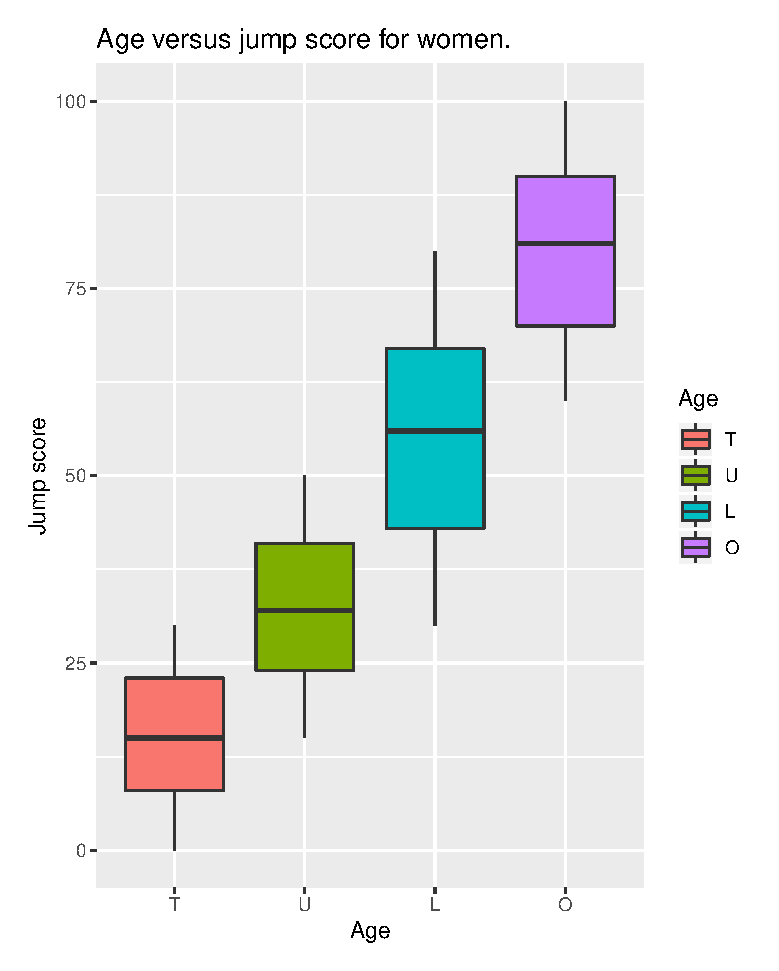
\includegraphics[width=\linewidth]{jumAgeWomen.eps} \vspace{-0.7cm} \caption{Each box-plot represents a different age group.} \label{jumAgeWomen} \par
    
    % Age distance %
    %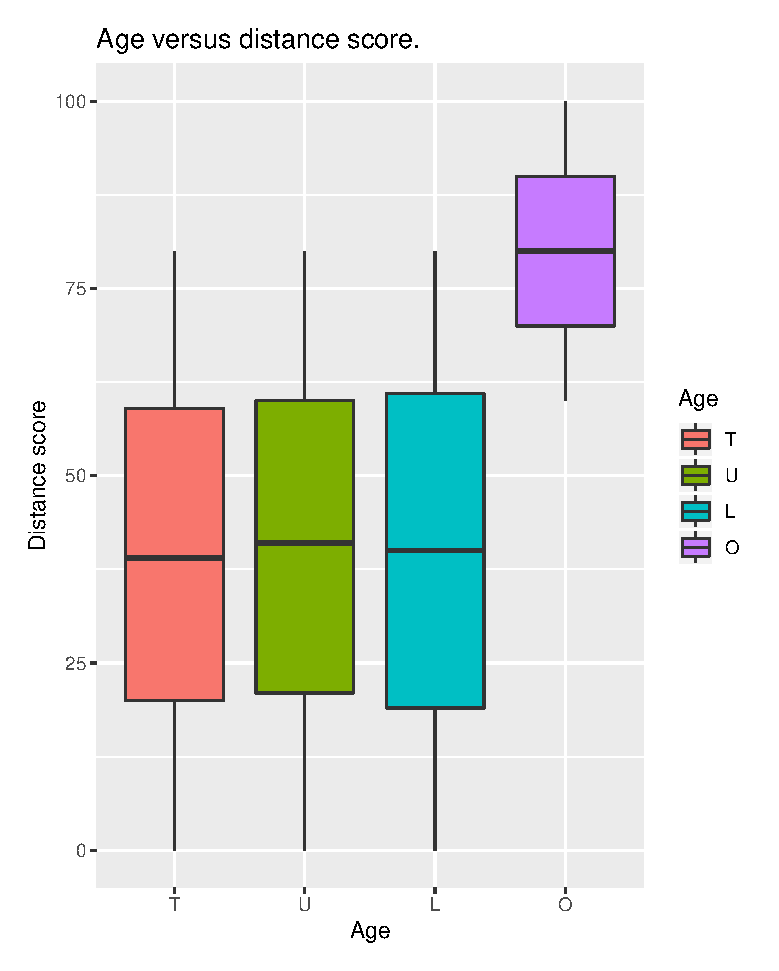
\includegraphics[width=\linewidth]{AgeDist.eps} \vspace{-0.7cm} \caption{The over 30s box plot, shown in purple, is above all of the others.} \label{ageDist} \par
%\end{multicols}   
%\begin{multicols}{2}
    % Overall location
 %   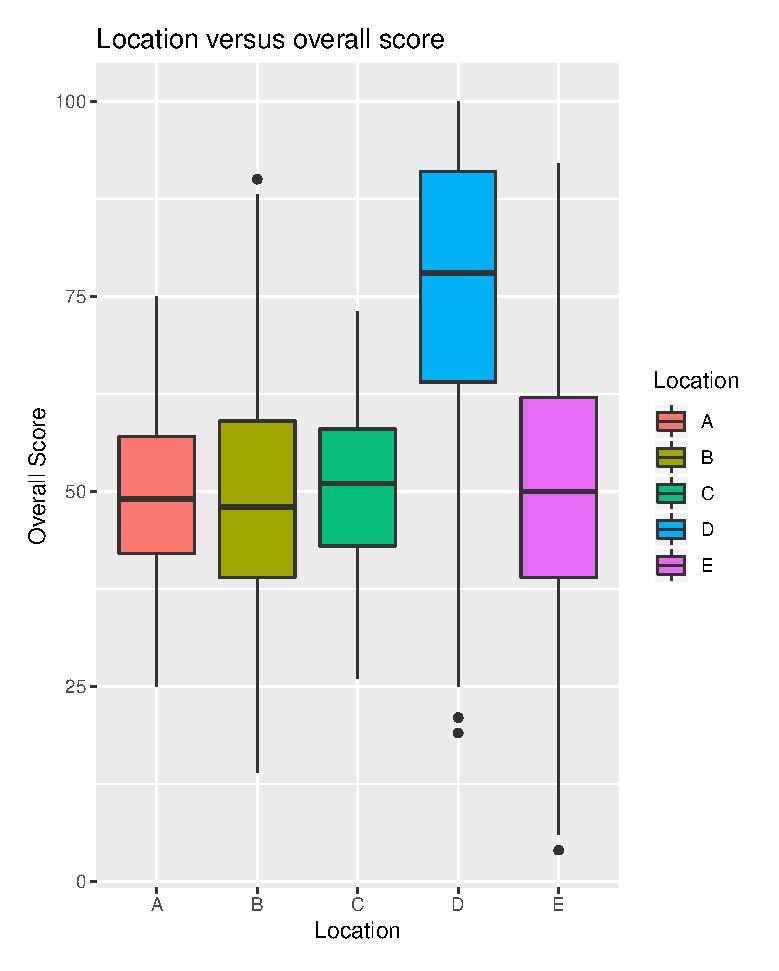
\includegraphics[width=\linewidth]{overLoc.eps} \vspace{-0.7cm} \caption{The blue box plot, representing location D, is higher than the others.} \label{overLoc} \par
    
    % Distance Jump Location A
  %  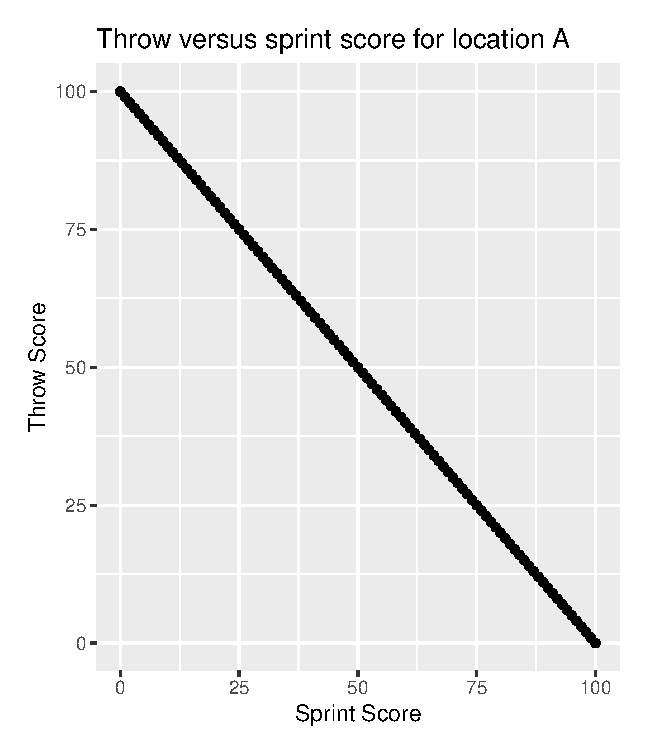
\includegraphics[width=\linewidth]{throwSprintLocA.eps} \vspace{-0.7cm} \caption{There is a 1:1 negative correlation between throw and sprint scores.} \label{throwSprintLocA} \par
%\end{multicols} 
%\end{figure}
%\begin{figure}
%\begin{multicols}{2}
    % Distance Jump Location B Men
 %   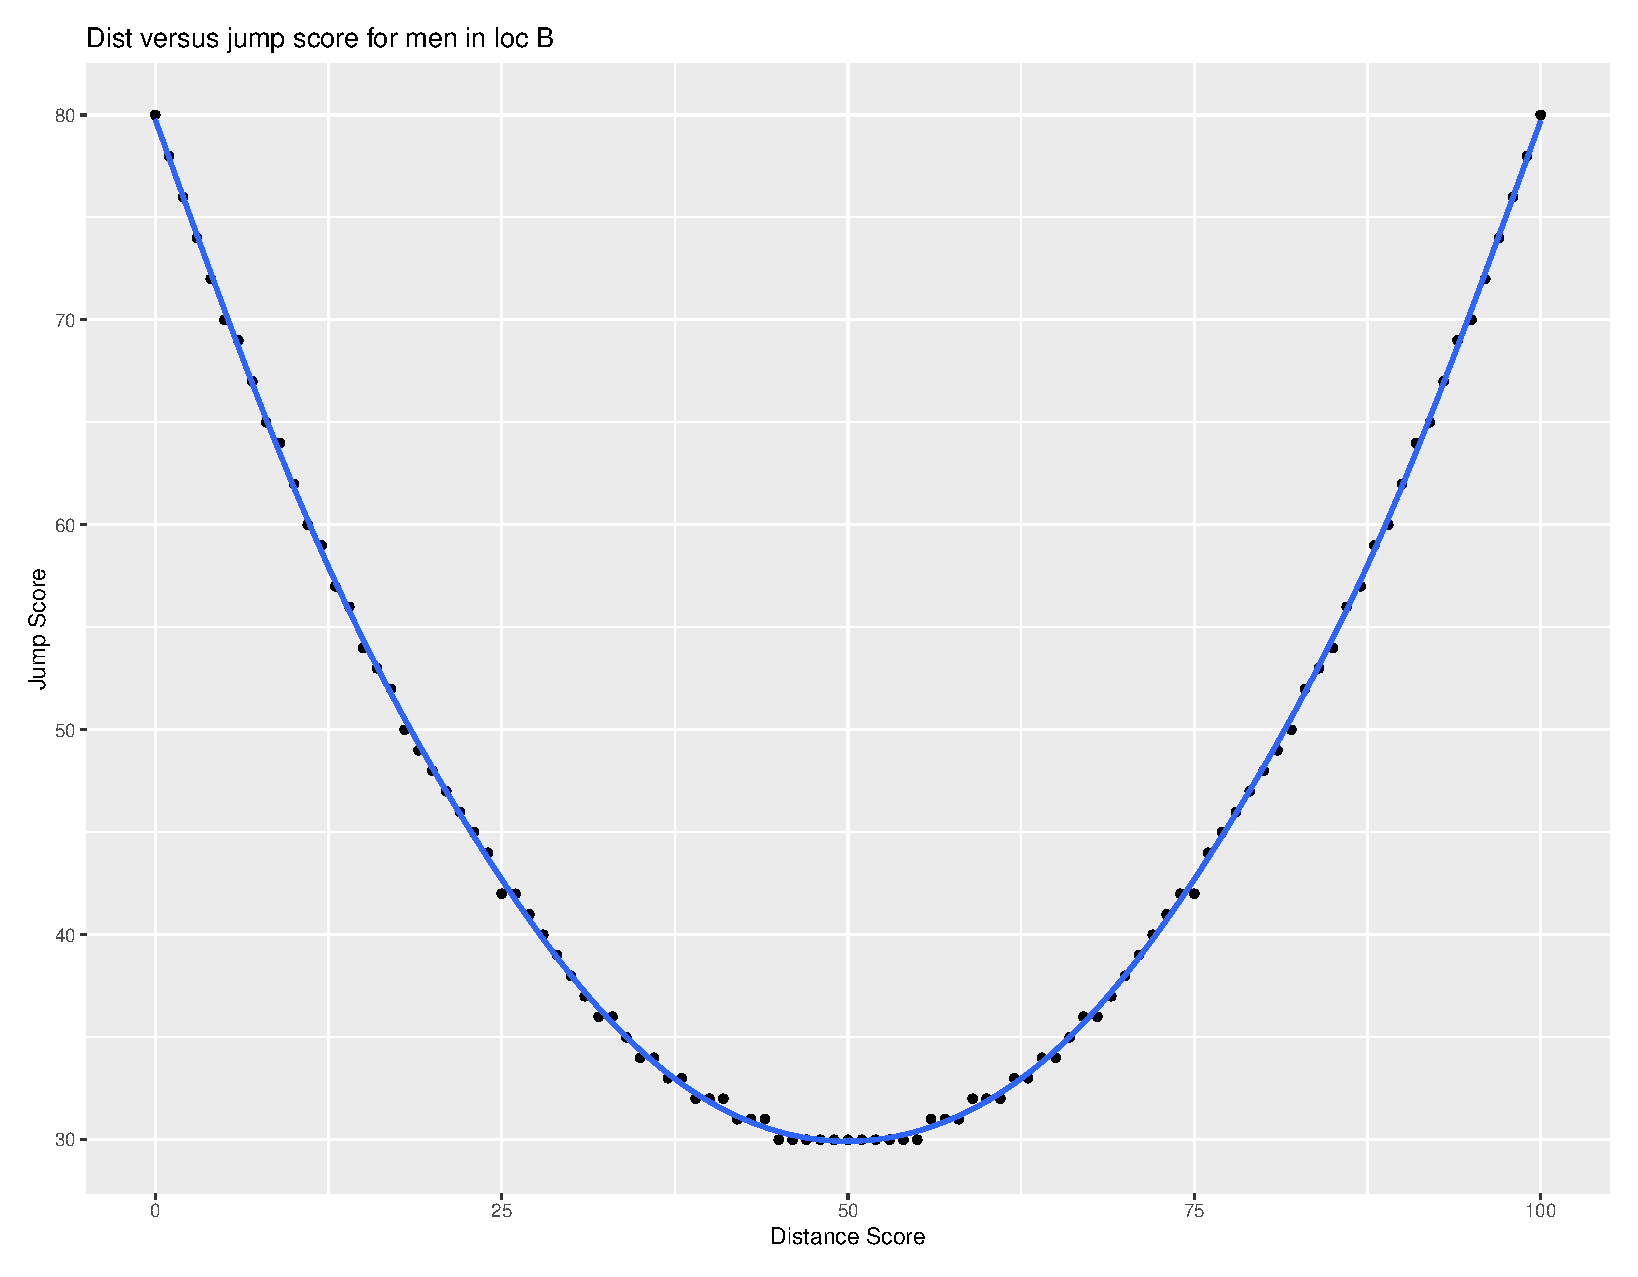
\includegraphics[width=\linewidth]{distJumpLocBMen.eps} \vspace{0cm} \caption{There is a quadratic relation between distance and jump scores.} \label{distJumpLocBMen} \par
    
    %Sprint jump Female Teen Location E
  %  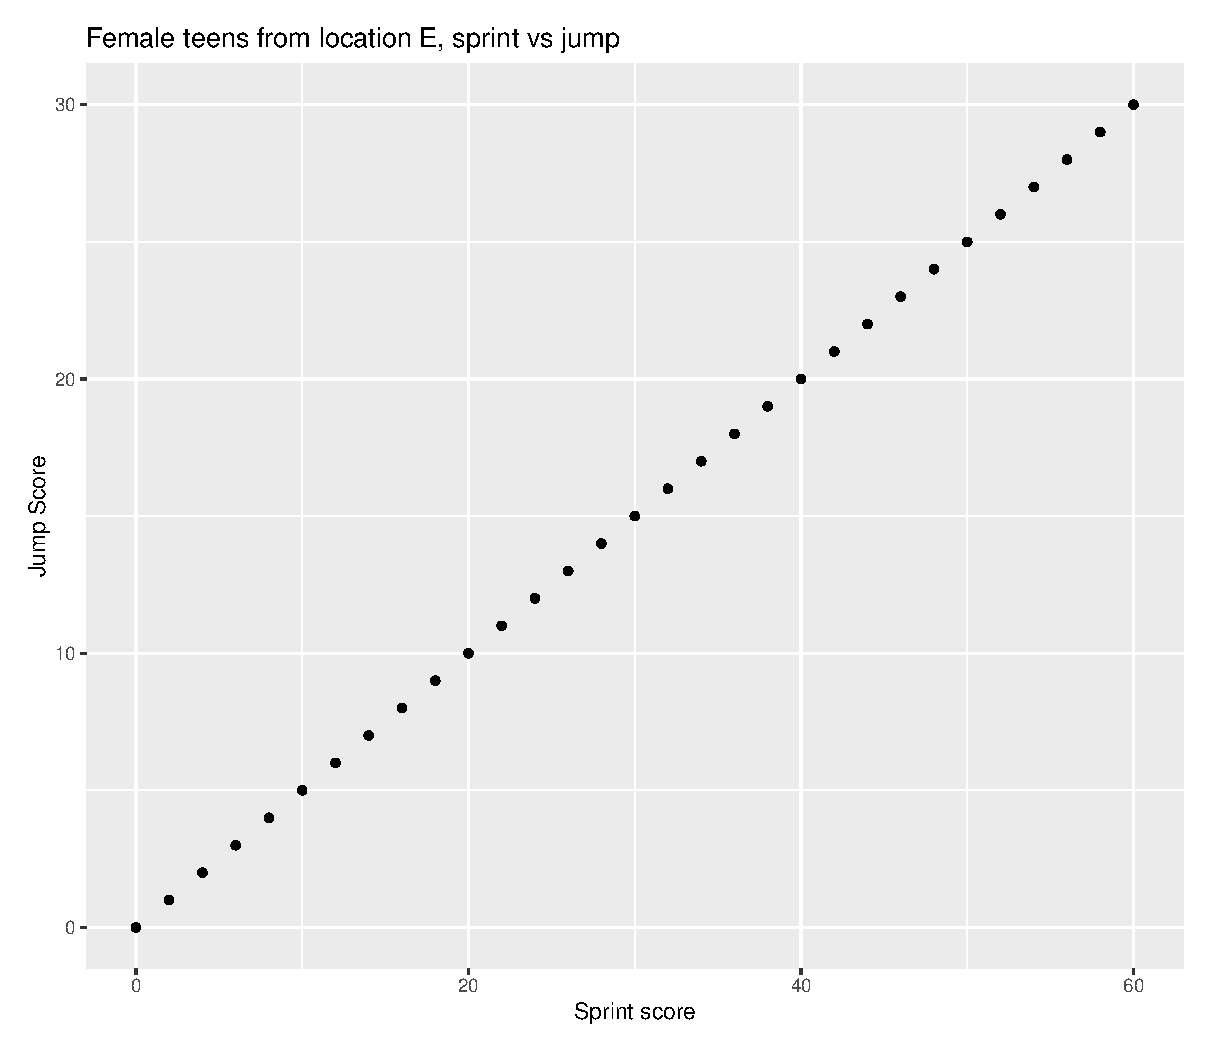
\includegraphics[width=\linewidth]{fTeSprintJump.eps} \vspace{-0.7cm} \caption{There is a strong positive correlation between sprint and jump for female teens in location E.} \label{fTeSprintJump} \par
%\end{multicols}
%\begin{multicols}{2}
    %Male Sprint Overall Facet Wrap
 %   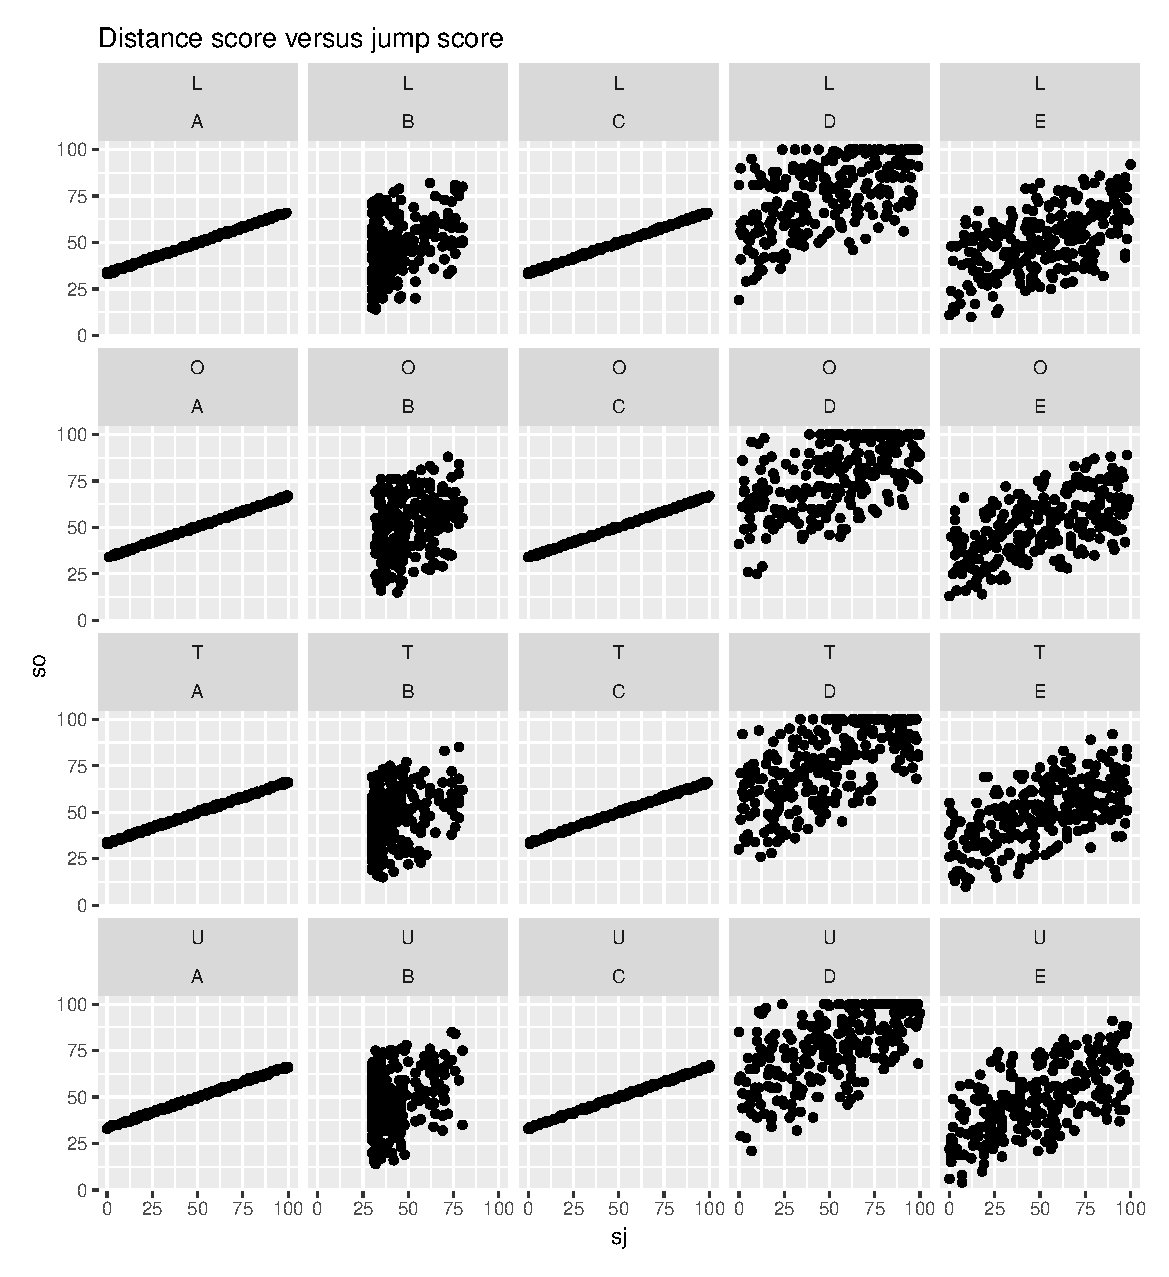
\includegraphics[width=\linewidth]{menACjumover.eps} \vspace{-0.8cm} \caption{There is a positive correlation between jump and overall scores for men, especially those from locations A and C.} \label{menACjumover} \par

    %Distance Jump Location B Men OPTIMIZED
  %  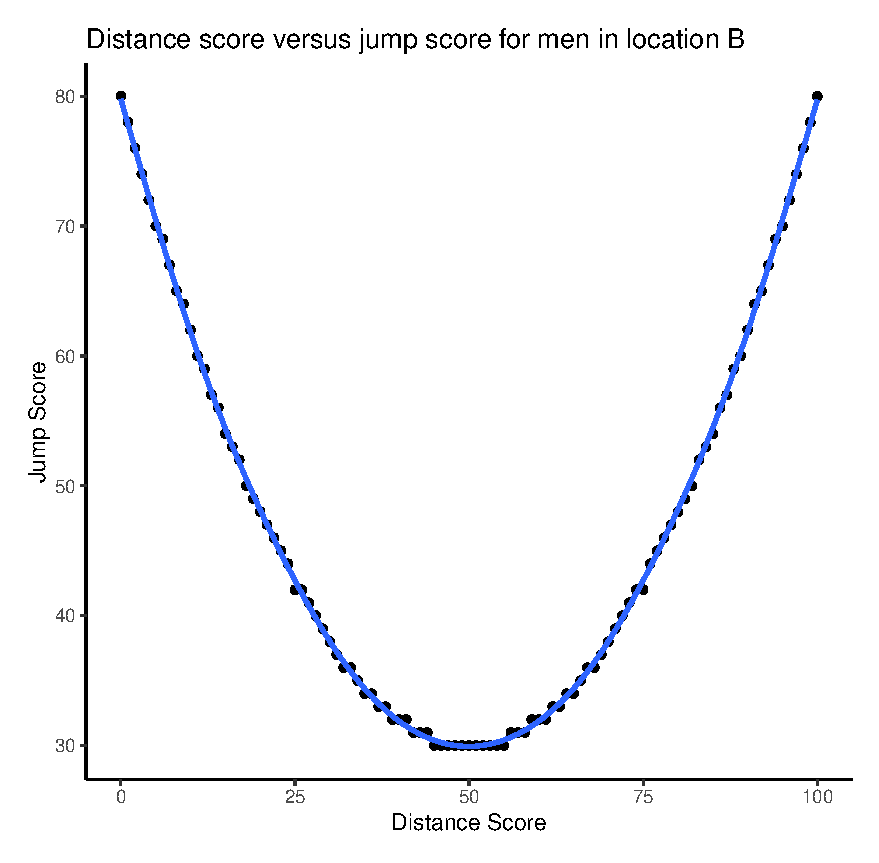
\includegraphics[width=\linewidth]{distJumpLocBMenOpt.eps} \vspace{-0.8cm} \caption{The optimized version of figure \ref{distJumpLocBMen}. As the original was already quite clear, I mostly focused on removing background elements for this optimized version.} \label{distJumpLocBMenOpt} \par

%\end{multicols}
%\end{figure}
%
% the environments 'definition', 'lemma', 'proposition', 'corollary',
% 'remark', and 'example' are defined in the LLNCS documentclass as well.
%
%\begin{proof}
%Proofs, examples, and remarks have the initial word in italics,
%while the following text appears in normal font.
%\end{proof}
%For citations of references, we prefer the use of square brackets
%and consecutive numbers. Citations using labels or the author/year
%convention are also acceptable. The following bibliography provides
%a sample reference list with entries for journal
%articles~\cite{ref_article1}, an LNCS chapter~\cite{ref_lncs1}, a
%book~\cite{ref_book1}, proceedings without editors~\cite{ref_proc1},
%and a homepage~\cite{ref_url1}. Multiple citations are grouped
%\cite{ref_article1,ref_lncs1,ref_book1},
%\cite{ref_article1,ref_book1,ref_proc1,ref_url1}.

\end{document}
